\chapter{函数}
\label{ch:Functions}
这一章节依旧是IGCSE的内容,不过再深入一点而已


\section*{学习目标}
\begin{todolist}
\item 理解函数,定义域,值域等相关术语
\item 理解反函数的概念,掌握求算方法
\item 掌握一对一函数及其反函数的图像特征
\item 理解复合函数的概念,并解决复合函数的相关问题
\item 理解并使用函数的变形和对应的标记手段
\end{todolist}
\clearpage

\section{映射与函数}
\label{sec:Mapping and function}
有没有想过,为什么先驱会把function这个翻译为功能的单词,再用作数学当中函数的概念?

\subsection*{映射}
\label{subsec:Mapping}
请看下图:

\begin{figure}[H]
\centering
\includegraphics[width=0.5\textwidth]{wife-husband}
\caption{娱乐圈中的妻夫关系}
\end{figure}

高圆圆的老公是赵又廷,孙俪的老公是邓超,谢楠的老公是吴京。于是在左侧的女生的女生\gls{set}当中的每一个\gls{elem}都与右侧男生集合中的一个元素对应起来了,于是在女生集合和男生集合之间就有一种\gls{mapping}。这种映射关系很明显就是夫妻关系,因此当再次输入一个已婚女性的名字进入到该映射关系中,其对应的合法丈夫的名字就会出现在男生集合中。又由于一夫一妻制,这种关系必须是一对一的关系。one-to-one

但是,再看下图当中:
\begin{figure}[H]
\centering
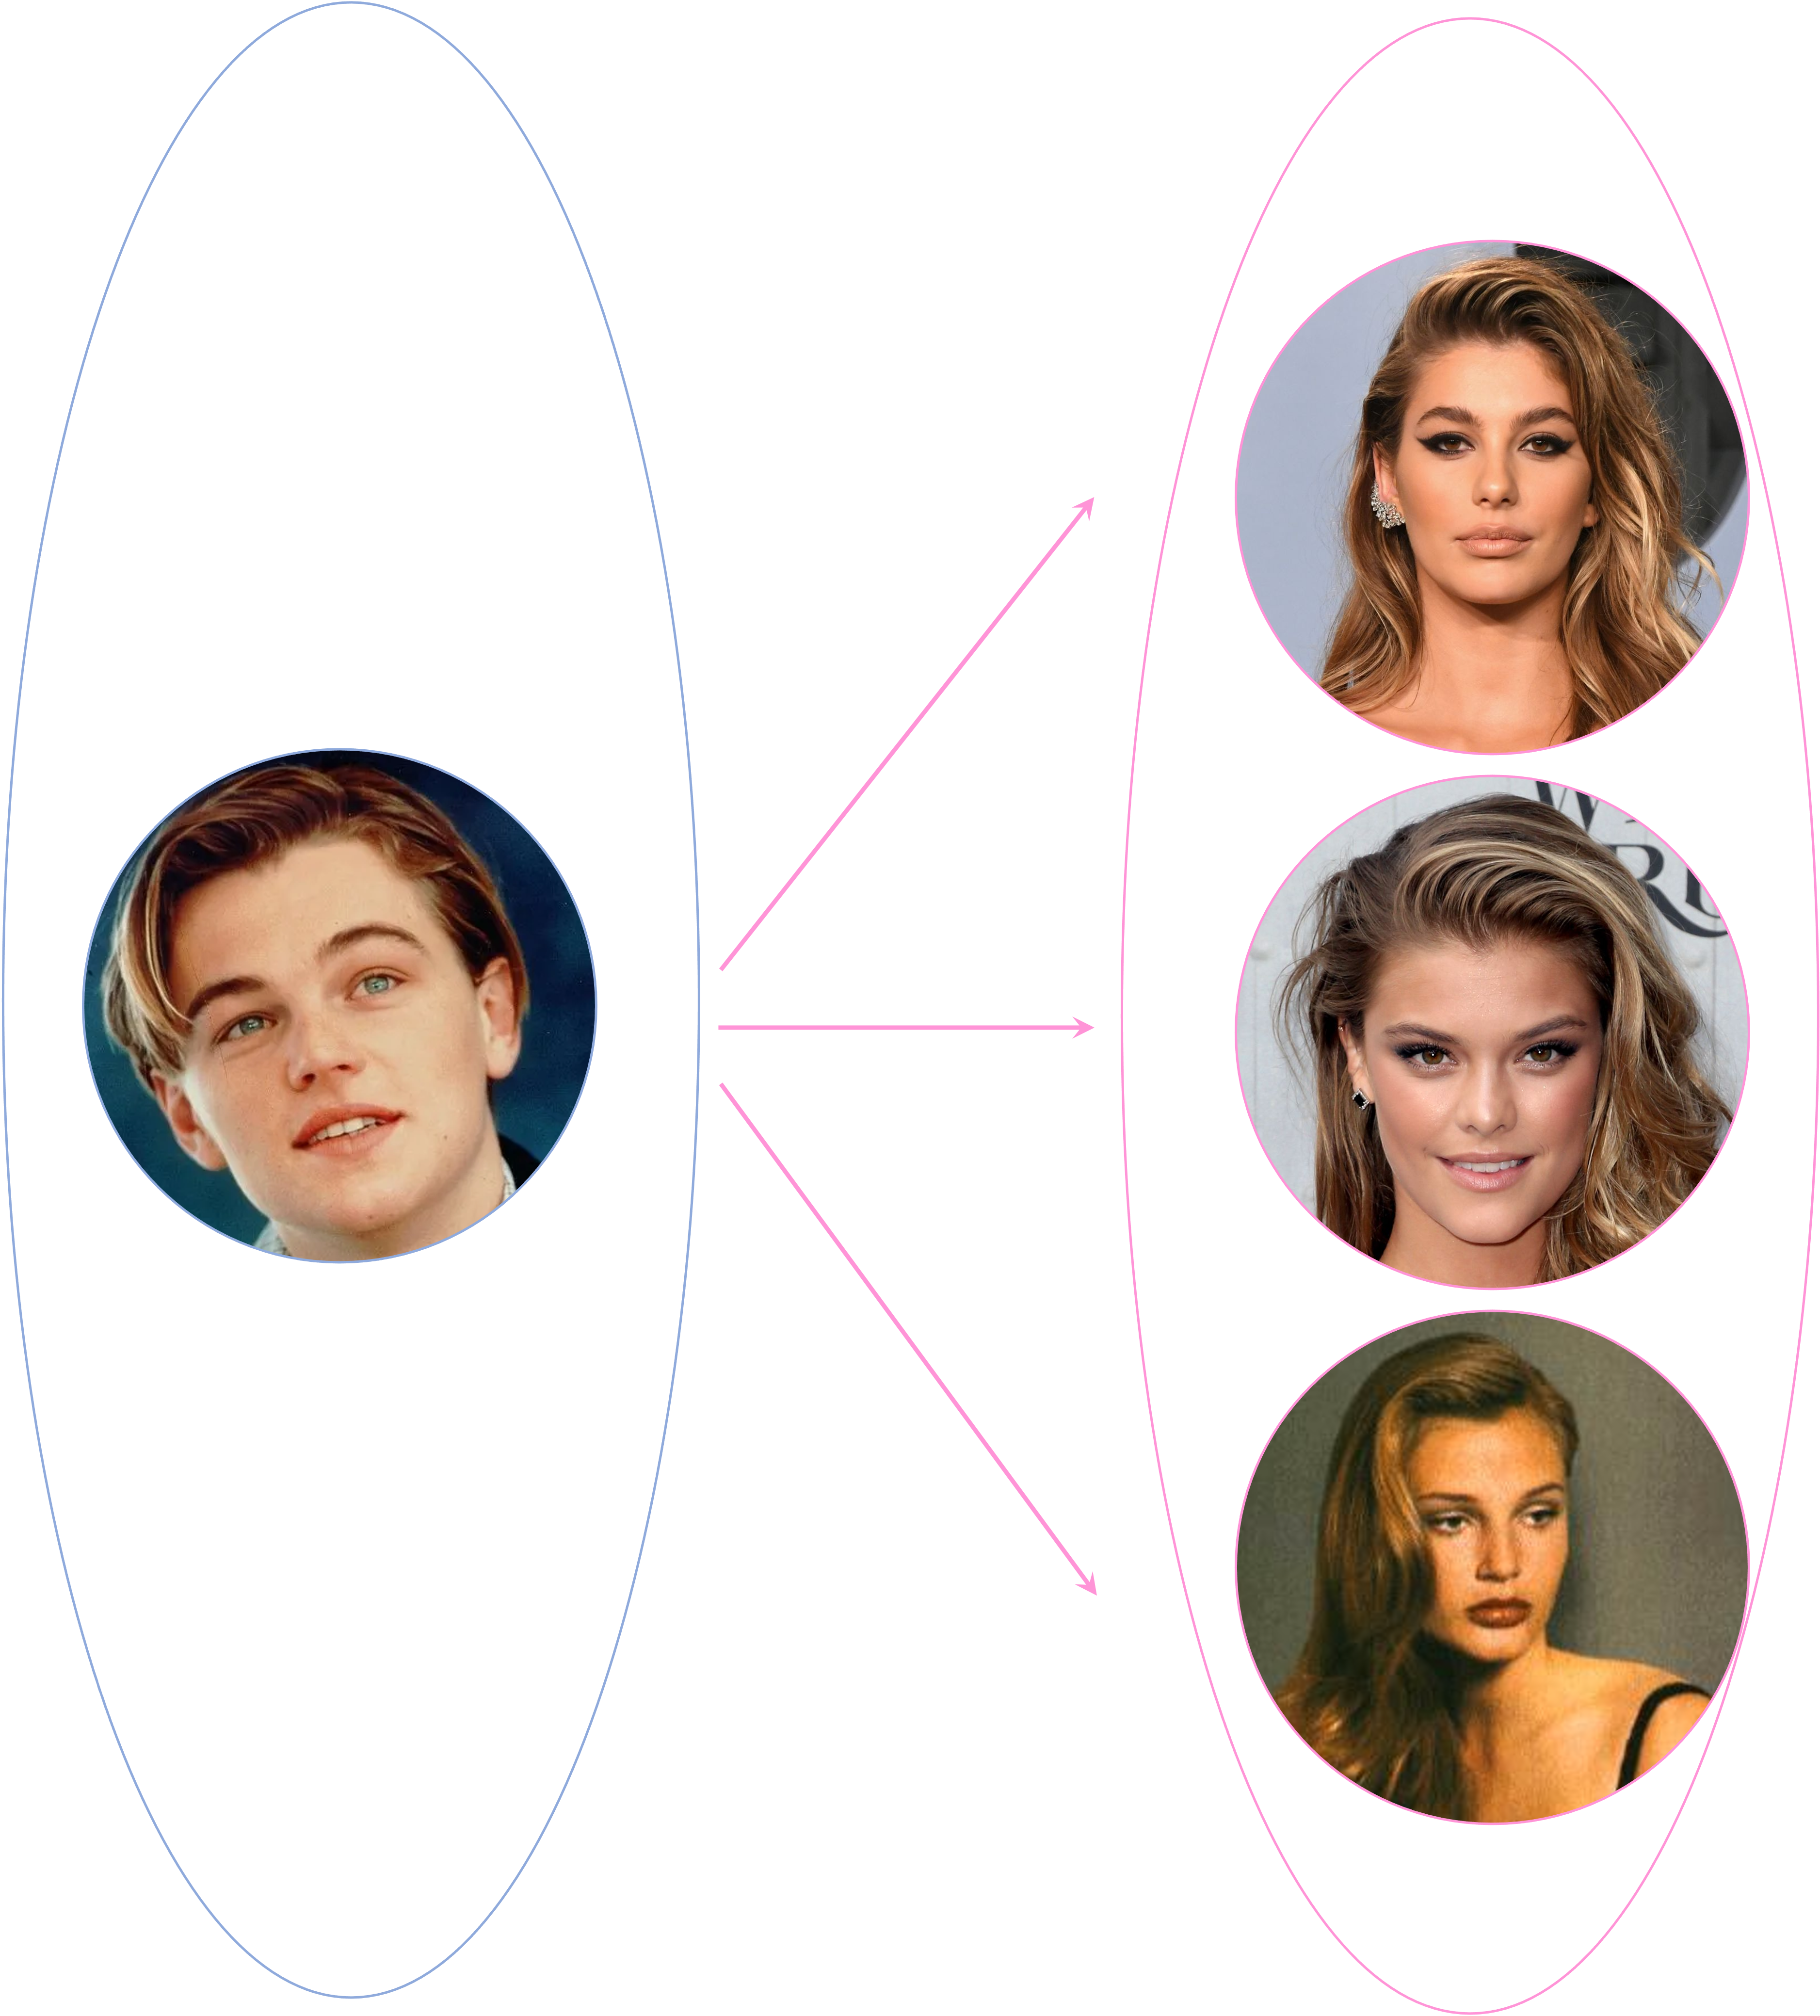
\includegraphics[width=0.5\textwidth]{Leonardo}
\caption{粗略统计Leonardo交往过20个女生}
\end{figure}

这也是一种映射,但是,左侧的一个元素对应着右侧多个元素。这种映射就是一对多的映射。

\subsection*{函数}
\label{subsec:Function}
上图的关系一对一关系就可以称之为是一种函数的。如果让$x$代表左边集合中的任意元素,$y$代表右边集合中的某一元素。那么我们就可以将这种函数关系记作如下的形式:
\[
	f: x\mapsto y  \qquad \text{or} \qquad  y=f(x)
\]
比如,上图当中的妻夫关系就可以计作$f(\text{高圆圆})=\text{赵又廷}$。但是很明显这样的表达式并不适合$f(\text{Leonard})$,等于号后面,填谁都不适合。因为这不是one-one relationship。

\subsubsection*{定义域与值域}
\label{Domain and Range}
当我们开始讨论数字集合的时候,集合中的元素开始变成数字的之后。$x$被我们称之为\gls{zbl},$y$称之为\gls{ybl}都是来自于两个数字集合的元素。在描述函数的时候,需要我们描述一下这两个集合的范围,其中$x$的范围被我们称之为\gls{domain}, $y$的范围被我们称之为\gls{range}。不过由于数字的运算特性,我们一般选择描述定义域就可以。可以通过函数的表达式确定出值域的大小。当然,考试的时候必定两个是可以互相求算的。

比如对于一个简单的二次函数:
\[
	y = x^2
\]
在这里不加任何限制的话,$x$可以选择带入任意实数数值,因此定义域为$x\in \mathcal{R}$。但是值域的话, $y$必定是非负数,因此值域可以计作$y\in [0,\infty)$。

但是如果考虑场景的话,比如$x$代表一个正方形的边长,$y$代表该正方形的面积。那么此时$x$作为一个长度就不能取到负值,并且边长为$0$的正方形也没太大意义。因此此时$x>0$就是这个函数的定义域了。
\clearpage


\section{反函数}
\label{sec:Inverse Function}
当我们考虑将左右侧的集合调换。形成如下图的映射:
\begin{figure}[H]
\centering
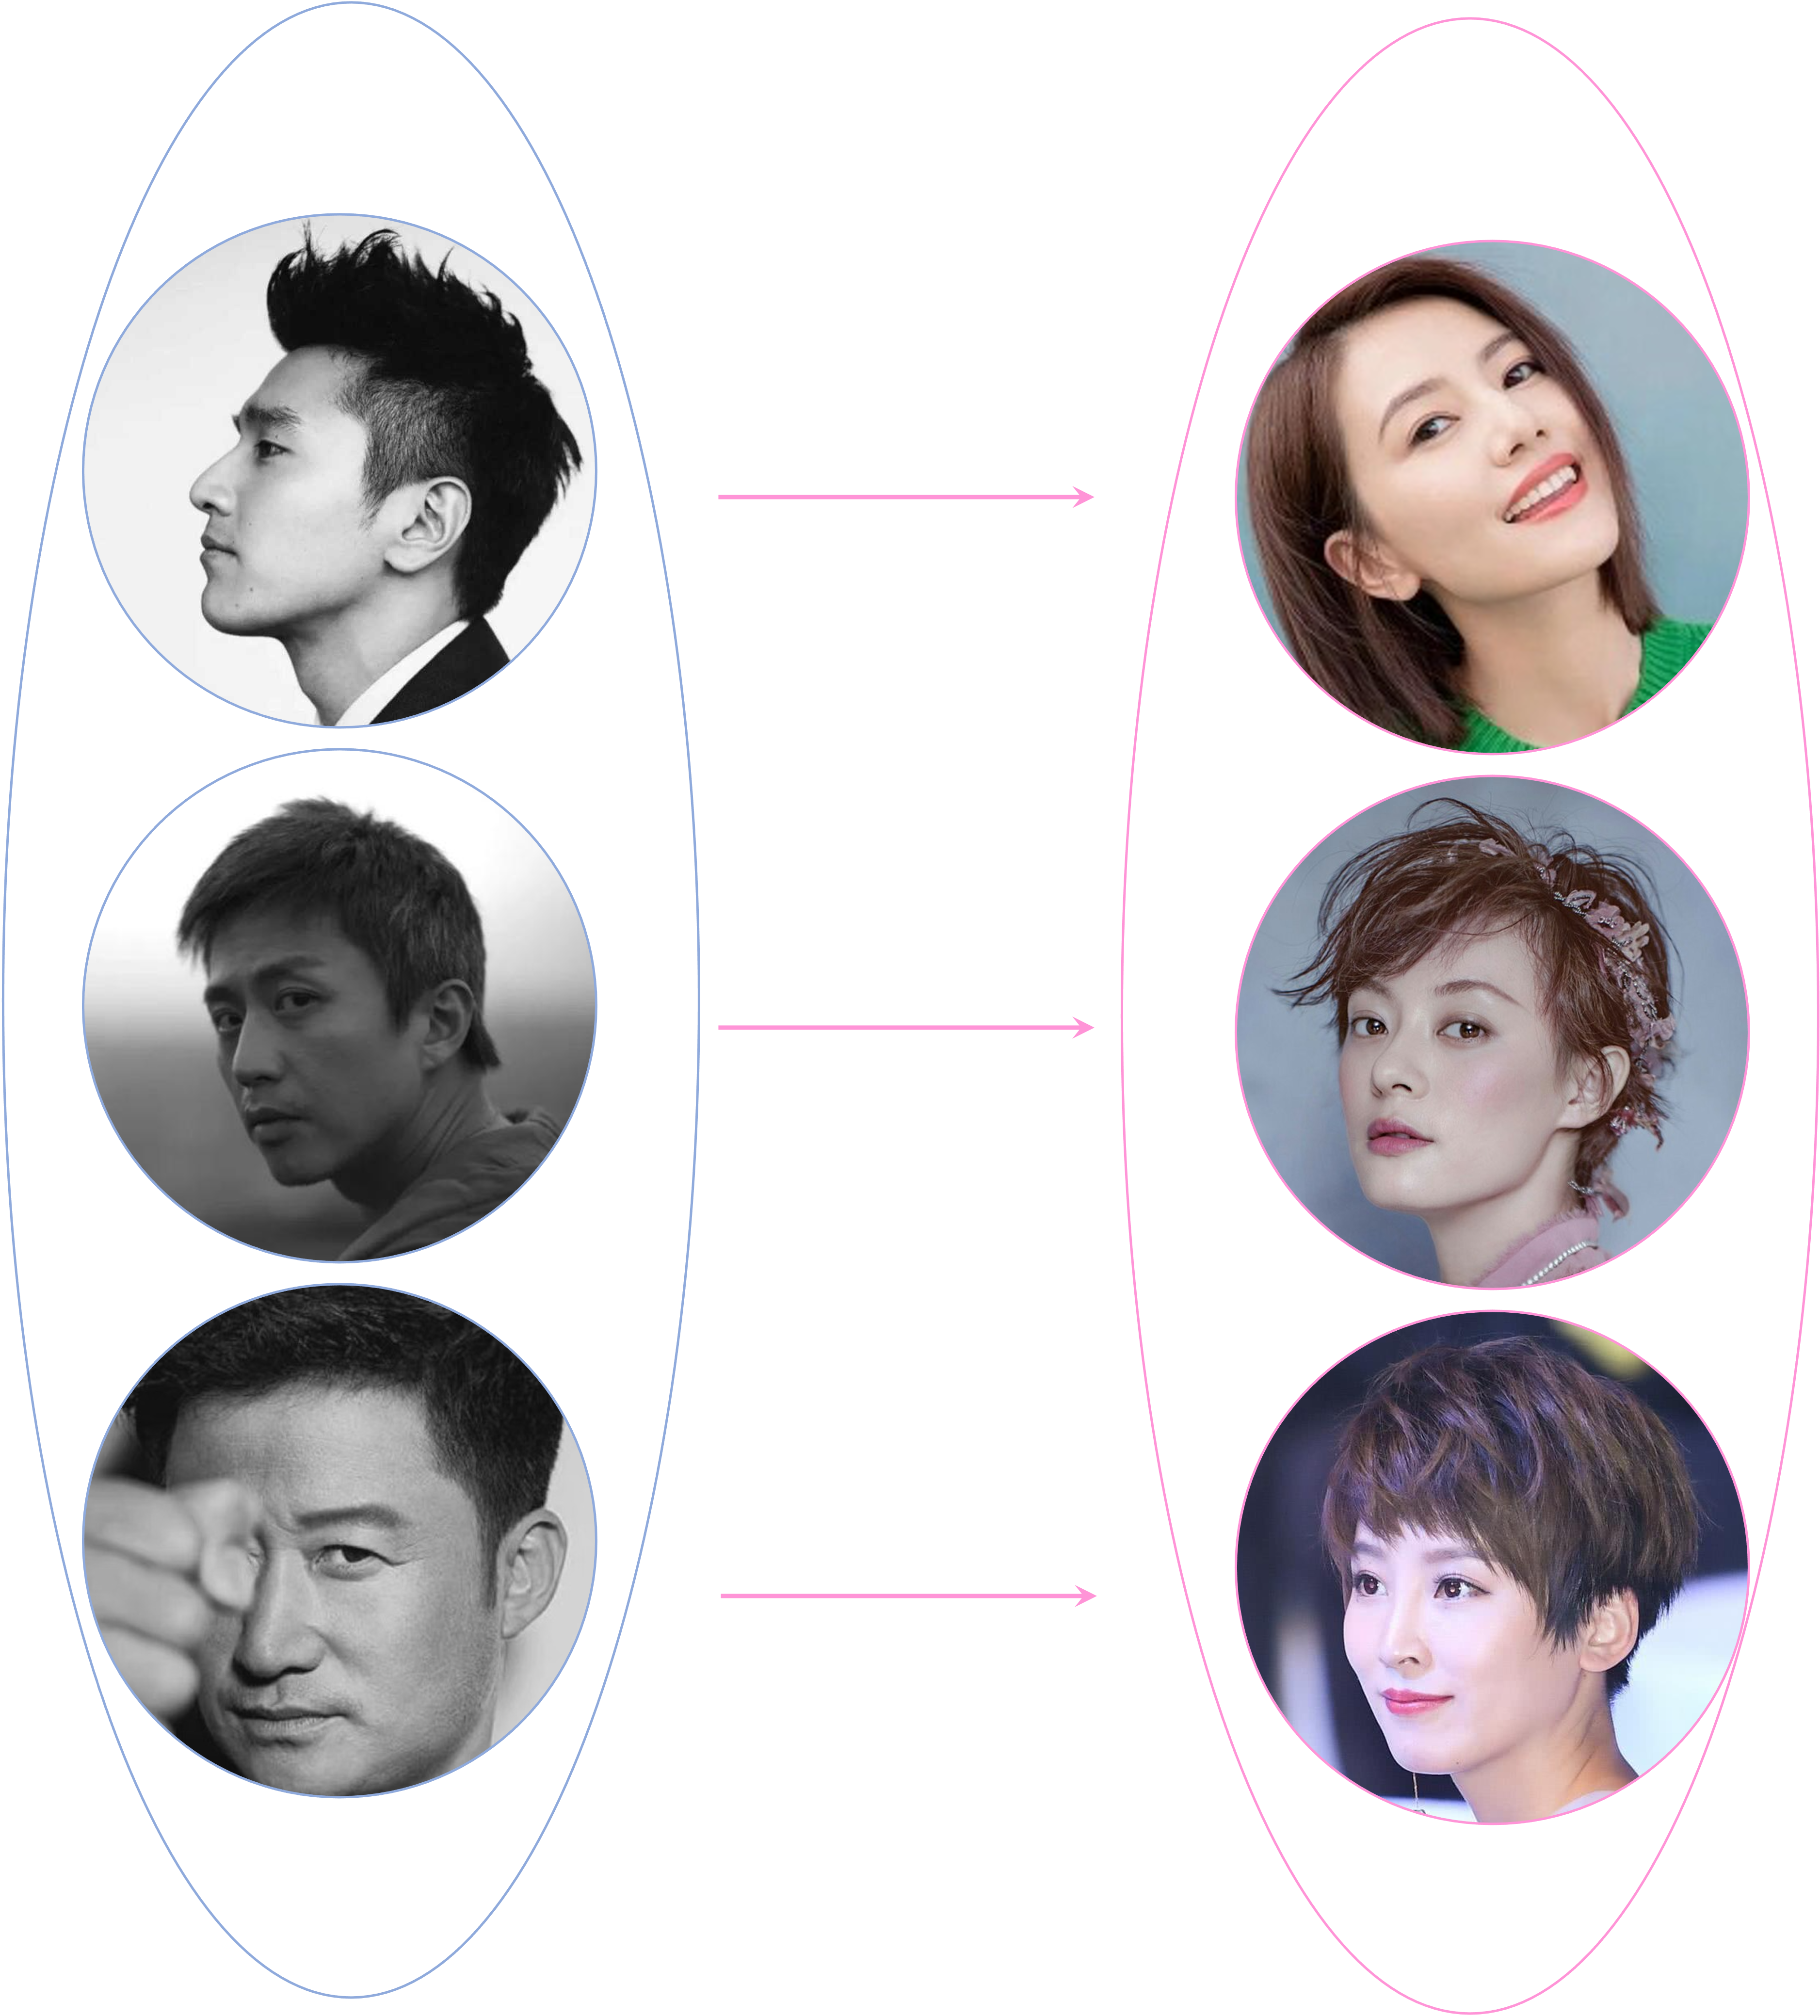
\includegraphics[width=0.5\textwidth]{husband-wife}
\caption{娱乐圈中的夫妻关系}
\end{figure}


赵又廷$\mapsto$高圆圆,邓超$\mapsto$ 孙俪, etc这些映射也是一对一的。因此必定也可以写作一个函数,之前已经确定了一个函数$f$,可以称之为找老公函数,那么这里就是它的\gls{inverse}。我们可以计作$f^{-1}$。当然如果不拘泥于这种写法的话,其实符号是可以任意选择的。比如$y=zlg(x)$ vs $y=zlp(x)$。只不过虽然这里两个函数的自变量都是$x$,但是取值的范围是完全不同的, 在$zlg$函数中,$x$的定义域是女生集合;但是在他的反函数$zlp$中,$x$的定义域是男生集合,恰好是原函数$zlg$中的值域。

\subsection*{能形成反函数的要求}
\label{subsec:Requirements}
由于反函数将原函数的值域作为自己的定义域。对于原函数,我们能确保,$x$只能对应一个$y$。但是对调之后这种关系可能不存在的了,如下面的函数
$h: x\mapsto (2x-3)^2-4$。当$x=1$或者$x=2$时,都对应着同样的$y=-3$。因此$h^{-1}(-3)$则陷入了和小李子一样的困境。不能满足one-one的要求,该函数则没有反函数。

\begin{SummBox}
能形成反函数,要求一个$x$有且只有一个$y$与之对应,与此同时,一个$y$值也只对应着一个$x$。
\end{SummBox}

\subsection*{确定反函数}
\label{subsec:Find Inverse}
对于上面的函数$y=h(x)=(2x-3)^2-4$,当我们把定义域稍作修改,从$x\in \mathcal{R}$ 改编成为$x>\frac{3}{2}$时,会满足了反函数存在的要求,因此就会有反函数存在了。那么如何确定这个反函数呢?

之前我们讨论过了,反函数交换了自变量和因变量。因此原函数的$x$现在成为了反函数中的$y$。原函数的$y$现在成为了反函数中的$x$。
比如$h(2)=-3$,那么$h^{-1}(-3)=2$。所以求算反函数只需要将表达式中的$x$,$y$对调一下就行了。
\[x=h(y)=(2y-3)^2-4\]
但是,我们希望得到的是$y=h^{-1}(x)$。因此需要再做一下整理化简:
\begin{align*}
x=h(y) &= (2y-3)^2-4\\
 x+4   &=(2y-3)^2\\
  2y-3 &=\sqrt {x+4} \quad \text{neglect negative value}\\
  y    &=\frac{\sqrt{x+4}+3}{2}\\
  y=h^{-1}(x) &=\frac{\sqrt{x+4}+3}{2}
\end{align*}

再陈述一下反函数$y=h^{-1}(x)$的定义域,$x>-4$就可以了

\begin{TaskBox}
$x>-4$是从哪里推导的?
\end{TaskBox}

\subsubsection*{反函数的图像特征}
\label{subsec:Graphic Charcteristic}
由于原函数和反函数的对应关系,最终会形成关于直线$y=x$对称的特征,并且如果原函数和反函数图像有交点的话,交点也只能在$y=x$图像上,思考一下为什么。

如下图所示,红线和蓝线就是两个互为反函数的图像。
\begin{figure}[H]
\centering
\includegraphics[width=0.8\textwidth]{inverse} %todo 原函数和反函数的图像
\caption{原函数和反函数的图像}
\end{figure}
\clearpage

\section{复合函数}
\label{sec:Composite Function}
\gls{comp}是将两个函数合并起来的函数。
比如:
\[f(x)=3x+2 \qquad g(x)=x^2+2x+4\]
那么: $fg(x)$则表示,将$x$首先带入到$g$函数中,然后再将得到的结果$g(x)$,代入到$f$函数中。等价于$f(g(x))=3\cdot g(x)+2$。

因此最后$fg(x)=3\cdot(x^2+2x+4)+2=3x^2+6x+14$。
在求算过程中需要注意,由于第一步要进行$g$函数的运算,因此$x$必须满足$g$的定义域;然后$g(x)$作为函数$f$的自变量,因此要满足$f$的定义域。这个点往往会被忽略掉。
\clearpage


\section{函数图像的变形}
\label{sec:Transformation of graphs}
当对一个函数进行简单的变形之后,也会对其图像产生一些变化。这些变化主要分为三大类。

\subsection*{平移}
\label{subsec:Translation}
对于一个函数$y=f(x)$而言,如果在原函数的基础上,改写为$y=f(x)+a$,构成一个新函数,那么这个新函数的图像会和原来的函数形状一模一样。只不过会从原函数的图像向\emph{上}\gls{py}$a$个单位(如果$a>0$)。向\emph{下}平移$a$个单位(如果$a<0$)。

原因如下:
假设$A$点的坐标为$(x_0,y_0)$,且满足$y_0=f(x_0)$,那么$A$点在原函数$y=f(x)$的图像上;假设$A'$点的横坐标与$A$点横坐标一致,且在$y=f(x)+a$上,那么$A'$点的坐标必定为$(x_0,y_0+a)$。也就意味着,$A'$点在竖直方向上与$A$点相差$a$个单位,如下图所示:
\begin{figure}[H]
\centering
\includegraphics[width=0.8\textwidth]{upshift.png}
\caption{图像在竖直方向上的平移}
\end{figure}

因此在一个函数表达式的最后加上或者减去某个数字带来的平行移动被我们称之为\emph{上加下减}。

但是接下来的概念会让很多人摸不着头脑,和之前相反。在水平方向上发生移动的规则被我们总结为\emph{左加右减}。也就是,如果$y=f(x+a)$这样的表达式会使新函数的图像出现在原函数的左边。

我们再重复刚才的一遍过程:
假设$A$点的坐标为$(x_0,y_0)$,且满足$y_0=f(x_0)$,那么$A$点在原函数$y=f(x)$的图像上;假设$A'$点的纵坐标与$A$点\emph{纵}坐标一致,且在$y=f(x+a)$上,那么此时,$A'$的横坐标求算要根据$y_0=f(x_0)$进行反推。由于$A'$是在新函数$y=f(x+a)$上的,因此可以写出:
\begin{align*}
y_0 &= f(x_0) \qquad \text{这是}A\text{点满足的关系}\\
y_0 &= f(x+a) \qquad \text{这是}A'\text{点满足的关系}\\
\end{align*}
对比之后,不难发现,$A'$点的横坐标等于$x_0-a$。而不像上下平移那样。因此$A'(x_0-a,y_0)$出现在$A(x_0,y_0)$的左侧(如果$a>0$),同理,整个新函数的图像会是原函数的图像向左边平移$a$个单位得到的。

\begin{figure}[H]
\centering
\includegraphics[width=0.8\textwidth]{leftshift}
\caption{图像在水平方向上的平移}
\end{figure}

\begin{SummBox}
左加右减,上加下减

$y=f(x+a)$ vs $y=f(x)+a$
\end{SummBox}


\subsection*{翻折}
\label{subsec:Reflection}
在这一小节中,我们将处理$y=-f(x)$与$y=f(-x)$的图像变形,这种结果是统称为翻折。

再次利用$A$与$A'$点的对应关系,对于$y=-f(x)$函数。$A(x_0,y_0)$在原函数上,那么当$A'$与$A$有一样的横坐标时,其纵坐标必定为$-f(x_0)=-y_0$。因此$A'$点与$A$点的关系是,横坐标相同,纵坐标互为相反数,当这种关系放在任意点上的时候,就能够使新函数与原函数的图像关于$x$轴对称,如下图所示
\begin{figure}[H]
\centering
\includegraphics[width=0.8\textwidth]{x-reflect}
\caption{沿$x$轴翻折的图像}
\end{figure}

同理,如果是$y=f(-x)$,由于此时是对$x$进行变形,因此$A'$点与$A$的关系是横坐标互为相反数,纵坐标相同,因此新函数与原函数的图像关于$y$轴对称,如下图所示
\begin{figure}[H]
\centering
\includegraphics[width=0.8\textwidth]{y-reflect}
\caption{沿$y$轴翻折的图像}
\end{figure}

\begin{SummBox}
$-f(x)$会使图像沿着$x$轴翻折;

$f(-x)$会使图像沿着$y$轴翻折。
\end{SummBox}

\begin{TaskBox}
如果是$-f(-x)$,新图像会发生什么样的变化
\end{TaskBox}

\subsection*{拉伸}
\label{subsec:Stretch}
这是考试当中最后一个函数图像的变形。$y=a\cdot f(x)$和$y=f(a\cdot x)$

还是一样,先看容易的。对整体表达式$f(x)$乘以$a$的运算操作。召唤老朋友$A(x_0,y_0)$和$A'$。由于$A'$的横坐标和$A$的横坐标一致,因此其纵坐标为$a\cdot f(x_0)=a\cdot y_0$刚好是$A$点坐标的$a$倍。而这样的结果是使得函数图像拉长(如果$a>1$),使得函数图像压扁(如果$0<a<1$)。就像膨胀或者缩小的气球一样。
\begin{figure}[H]
\centering
\includegraphics[width=0.8\textwidth]{expandingballoon}
\caption{绘制在气球上的函数图像会被拉伸}
\end{figure}

当然,上面图是帮助理解,下面的这张图才是真正Stretch by a factor greater than 1 or less than 1的图像:
\begin{figure}[H]
\centering
\includegraphics[width=0.4\textwidth]{stretch-v}
\includegraphics[width=0.4\textwidth]{compress-v}
\caption{竖直方向上的拉伸与压缩} %有可能会报错
\end{figure}


第二种,在水平方向上的拉伸与压缩,要靠$y=f(ax)$进行实现。召唤老朋友$A(x_0,y_0)$和$A'$。由于$A'$点和$A$点的\emph{纵}坐标保持一致。于是得到:
\begin{align*}
y_0 &= f(x_0) \qquad \text{这是}A\text{点满足的关系}\\
y_0 &= f(a\cdot x) \qquad \text{这是}A'\text{点满足的关系}\\
\end{align*}

那么显然$A'$的横坐标只能是$\frac{x_0}{a}$。因此新的对应点$A'(\frac{x_0}{a}, y_0)$会与原始点保持纵坐标相同,横坐标被压缩(如果$a>1$)或者拉伸(如果$0<a<1$)。其结论还是和竖直方向上的结论相反。
\begin{figure}[H]
\centering
\includegraphics[width=0.4\textwidth]{stretch-h}
\includegraphics[width=0.4\textwidth]{compress-h}
\caption{水平方向上的拉伸与压缩} %有可能会报错
\end{figure}

\begin{SummBox}
$y=af(x)$会使图像在\emph{竖直}方向上进行拉伸,如果$a>1$,图像会被拉长$a$倍;如果$0<a<1$则会使图像压缩$\frac{1}{a}$倍;

$y=f(ax)$会使图像在\emph{水平}方向上进行拉伸,如果$a>1$,图像会被压缩$a$倍;如果$0<a<1$则会使图像拉长$\frac{1}{a}$倍;
\end{SummBox}


\subsection*{变形的结合}
\label{subsec:Combination of Transformation}
考试不会如此仁慈地只讨论一种变形,在表达式中常常会将多种变形结合在一起,重要的是能够确定执行那些操作,以及这些操作的量。

比如

1. $y=-3f(x)$ 

明显就是可以先操作$y=3f(x)$,也就是竖直方向上拉伸$3$倍,再执行关于$x$轴的翻折

2. $y=f(2x+4)$

方法1:\\
先进行平移的向左边移动$4$个单位得到$y=f(x+4)$;再进行水平方向上的压缩,$2$倍;

方法2:\\
先进行水平方向上的压缩,$2$倍得到$y=f(2x)$;注意,此时无需再向左边移动$4$个单位,而是仅仅移动$2$个单位。原因是:此时$x$作为整体,当向左平移$2$个单位的时候,表达式变成$y=f(2\boxed{(x+2)})=f(2x+4)$。因此如果使用先拉伸压缩,再平移量的方法,平移量会受到系数的影响。需要牢记。

在该\href{https://www.desmos.com/calculator/6yzdqimnlc}{Shift and Transformation}中有所有三种变形的情况,多调整一下滑块
体会一下这三种变动。




